\chapter{Codifica}
\label{cap:codifica}

\intro{In questo capitolo viene descritto il processo di codifica del progetto di stage.}

\section{Codifica back-end}

In questo capitolo verrà descritto il processo di codifica \emph{back-end} del
progetto di stage. Verranno elencate tutte le funzionalità e la struttura del
codice implementato.

\subsection{Config}

All'interno di questa cartella è presente il file di configurazione utilizzato
dal servizio. Di seguito la descrizione dello stesso.

\subsubsection{\emph{config.go}}

Questo file contiene la configurazione necessaria al funzionamento del servizio.
Esso contiene al suo interno le variabili d'ambiente che verranno utilizzate
dalla funzione \emph{Lambda} per recuperare i nomi delle tabelle \emph{DynamoDB}
e i nomi dei \emph{bucket S3} dove verranno recuperate e salvate le immagini.

\subsection{Clients}

All'interno di questa cartella è presente il file che definisce le funzioni per
utilizzare i \emph{client} di \emph{DynamoDB} e \emph{S3}.

\subsubsection{\emph{clients}}

Questo file contiene le funzioni per utilizzare i \emph{client} di
\emph{DynamoDB} e \emph{S3}. Si dividono in funzioni \emph{remote} e
\emph{local}, più nello specifico:
\begin{itemize}
    \item \textbf{remote}: funzioni che utilizzano i \emph{client} di
          \emph{DynamoDB} e \emph{S3} per recuperare e salvare i dati nell'ambiente
          \emph{sandbox}. Queste funzioni utilizzano la configurazione di
          \emph{default} per accedere ai servizi \emph{AWS};
    \item \textbf{local}: funzioni che utilizzano i \emph{client} di
          \emph{DynamoDB} e \emph{S3} per recuperare e salvare i dati nell'ambiente di
          \emph{test} in locale. Queste funzioni utilizzano una configurazione vuota,
          senza credenziali, che punta ad un \emph{endpoint} locale.
\end{itemize}

\subsection{Cmd}

All'interno di questa cartella è presente il file che definisce le funzioni per
avviare la \emph{Lambda}.

\subsubsection{\emph{main}}

Questo file contiene la struttura che definisce un evento di conversione, nello
specifico è così rappresentata:
\begin{lstlisting}[language=go]
    type ImageConversionEvent struct {
        Filename string `json:"filename"`
	ClientID string `json:"clientID"`
    }
\end{lstlisting}

\captionof{lstlisting}{Struttura di un evento di conversione}

Nello specifico vengono definiti:
\begin{itemize}
    \item \textbf{Filename}: nome del file da convertire;
    \item \textbf{ClientID}: identificativo del cliente che ha richiesto la
          conversione.
\end{itemize}
Entrambi vengono recuperati da un file \emph{JSON} che viene passato alla
funzione \emph{Lambda}: questo file nel progetto di stage viene inserito
manualmente, in un ambiente di produzione verrà fornito da un servizio
esterno.\\
Nella funzione \emph{main} viene recuperata la configurazione desiderata e
vengono istanziati i \glsfirstoccur\gls{DAO}, gli oggetti che permettono di
interagire con i servizi \emph{S3} e \emph{DynamoDB}. Successivamente viene
inizializzato il servizio che effettua la conversione delle immagini e viene
passato alla funzione \emph{Lambda}.

\subsection{DAL}

All'interno di questa cartella sono presenti i file che gestiscono gli accessi
agli oggetti presenti nei \emph{bucket S3} e nei \emph{database DynamoDB}.

\subsubsection{\emph{client configuration DAO}}

Questo file contiene la struttura che definisce un \emph{DAO} per il recupero di
una configurazione di un cliente. Con il \emph{DAO} si aggiunge un livello di
astrazione tra due parti di una applicazione che devono lavorare a stretto
contatto, restando indipendenti l'una dall'altra.\\
Questo \emph{design pattern} permette inoltre di separare la logica di accesso
ai servizi con cui si interfaccia, così nel caso in cui si volesse cambiare il
servizio sottostante si dovrà solamente cambiare il \emph{DAO} e non l'intera
applicazione. La struttura di una configurazione è la seguente:
\begin{lstlisting}[language=go]
type ClientConfiguration struct {
        ConfigurationName string `dynamodbav:"ConfigurationName"`
        Width   string `dynamodbav:"Width"`
        Height  string `dynamodbav:"Height"`
        Quality int    `dynamodbav:"Quality"`
    }
\end{lstlisting}
L'attributo \emph{dynamodbav} permette al \emph{client} di \emph{DynamoDB} di
mappare i campi della struttura con i campi della tabella.\\

\subsubsection{\emph{conversions bucket DAO}}

Questo file contiene la struttura che definisce un \emph{DAO} per effettuare il
\emph{download} e l'\emph{upload} di un file da un \emph{bucket S3}. La funzione
di \emph{download} prende in input tre parametri:
\begin{itemize}
    \item \textbf{clientID:} identificativo del cliente che ha richiesto la
          conversione;
    \item \textbf{jobID:} identificativo della conversione;
    \item \textbf{filename:} nome del file da scaricare.
\end{itemize}

Viene individuato il file all'interno del \emph{bucket S3} delle immagini da convertire, che si trova nella
cartella specificata dal \emph{clientID}. Successivamente viene effettuata una
copia del file in un percorso locale e viene restituito il percorso del file
appena salvato.\\

La funzione di \emph{upload} prende in input due parametri:
\begin{itemize}
    \item \textbf{clientID:} identificativo del cliente che ha richiesto la
          conversione;
    \item \textbf{filename:} nome del file da caricare.
\end{itemize}
Grazie a questi due parametri viene effettuato il caricamento del file nel
\emph{bucket} destinato alle immagini convertite.

\subsubsection{\emph{image conversion jobs DAO}}

Questo file contiene la struttura che definisce un \emph{DAO} per inserire le
specifiche di una conversione oppure per aggiornarle. La struttura di una
conversione è la seguente:
\begin{lstlisting}[language=go]
    type ImageConversionJob struct {
        ClientID       string `dynamodbav:"ClientID"`
        CreationDate   int64  `dynamodbav:"CreationDate"`
        ContentType    string `dynamodbav:"ContentType"`
        JobID          string `dynamodbav:"JobID"`
        EndDate        int64  `dynamodbav:"EndDate"`
        Status         Status `dynamodbav:"Status"`
        SourcePath     string `dynamodbav:"SourcePath"`
        TotalTime      int64  `dynamodbav:"TotalTime"`
        ConversionTime int64  `dynamodbav:"ConversionTime"`
        ErrorCause     string `dynamodbav:"ErrorCause"`
    }
\end{lstlisting}

Vengono salvate tutte le informazioni riguardanti la conversione, nello
specifico vengono salvati:
\begin{itemize}
    \item \textbf{ClientID:} identificativo del cliente che ha richiesto la
          conversione;
    \item \textbf{CreationDate:} data di inizio della conversione;
    \item \textbf{ContentType:} formato del file da convertire;
    \item \textbf{JobID:} identificativo della conversione;
    \item \textbf{EndDate:} data di fine della conversione;
    \item \textbf{Status:} stato della conversione. Può assumere tre valori: \emph{RUNNING}, \emph{COMPLETE} e \emph{ERROR};
    \item \textbf{SourcePath:} percorso del file da convertire;
    \item \textbf{TotalTime:} tempo totale della conversione, compreso il tempo
          di \emph{download} e \emph{upload};
    \item \textbf{ConversionTime:} tempo di conversione;
    \item \textbf{ErrorCause:} causa dell'errore, se presente.
\end{itemize}

Un esempio di come viene visualizzato un \emph{job} all'interno del
\emph{database DynamoDB} è il seguente:
\begin{figure}[H]
    \centering
    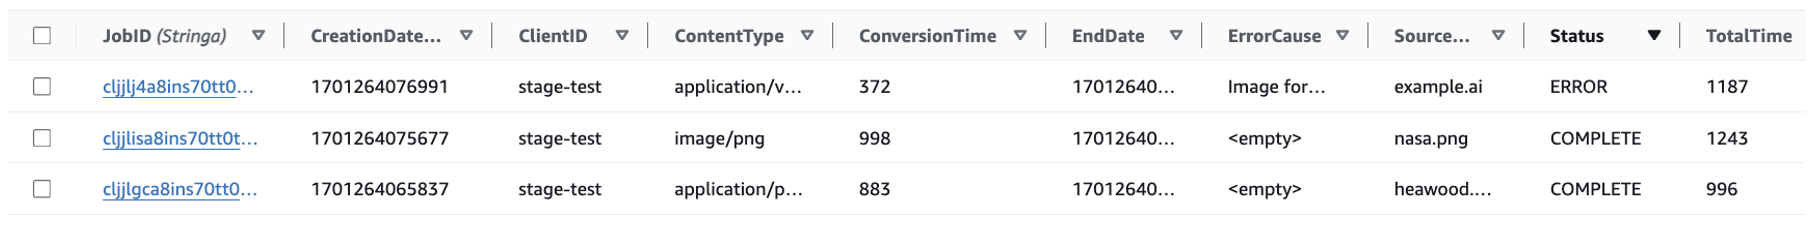
\includegraphics[width=1\textwidth]{images/esempio-job-dynamo.png}
    \caption{Esempio di un \emph{job} all'interno del \emph{database DynamoDB}}
\end{figure}

\subsection{Service}

In questa cartella viene definito il file principale del servizio, che contiene
il flusso di conversione delle immagini.

\subsubsection{\emph{image conversion service}}

In questo file viene definito tutto il flusso di conversione dell'immagine che
verrà poi gestito dalla \emph{Lambda}.\\
Sono state definite delle strutture che contengono tutti i formati gestiti dal
servizio, suddivisi per libreria che gestisce la conversione. Questi vengono
utilizzati per effettuare i controlli utilizzati come guardia per scegliere la
conversione adatta al formato richiesto. Per accelerare il processo di
conversione, seguendo il principio \emph{fail fast}, se il formato in ingresso
non è presente nelle strutture viene interrotto il flusso e viene restituito un
errore. Nella tabella contenente i \emph{job} di conversione, sarà presente
anche un campo dedicato a mostrare la causa dell'errore avvenuto.\\
Se il formato è accettato, viene verificato se è in atto un tentativo di
\emph{upscaling} dell'immagine, confrontando le dimensioni dell'immagine con
quelle richieste dalla configurazione: se sta per essere effettuato, viene
saltata la conversione per quel formato e viene restituito un messaggio di
\emph{warning} per avvisare che quella conversione non verrà eseguita.\\
Viene effettuata la conversione utilizzando il metodo adatto al formato in
ingresso ed infine viene caricata l'immagine nel \emph{bucket} di output ed
aggiornata la tabella contenente i \emph{job} delle conversioni.\\


\subsection{Utils}

In questa cartella è definito un file che contiene le funzioni di utilità che
sono state sfruttate in tutto il progetto.

\subsubsection{\emph{utils}}

In questo file sono presenti le funzioni che devono svolgere compiti ripetitivi
e per offrire metodi più semplici di interagire con altri programmi. Ogni
funzione, se non specificato diversamente, ritorna sempre un errore nel caso in
cui le operazioni richieste non vadano a buon fine. Le funzioni
definite sono le seguenti:
\begin{itemize}
    \item \emph{ExecuteCommand:} questa funzione permette di eseguire un
          comando come se si fosse in un terminale, specificando il nome del
          programma da utilizzare e i parametri da passare. Viene utilizzata ogni
          volta che vengono invocati i programmi esterni alle librerie di \emph{Go};
    \item \emph{CheckUpscaling:} questa funzione permette di verificare se le
          immagini di input sono più piccole di quelle richieste in output. Se
          si sta per verificare un caso di \emph{upscaling}, viene
          \emph{loggato} un messaggio di \emph{warning} e viene ritornato un
          errore specifico;
    \item \emph{CheckFormat:} questa funzione ha lo scopo di verificare se il
          formato \glsfirstoccur\gls{mimetype}, che le viene passato come
          stringa, sia presente nella struttura contenente i formati accettati
          da una specifica conversione. Questa funzione viene riutilizzata per
          ogni formato e permette di identificare nella lista di stringhe,
          rappresentata come \emph{mappa}, se la chiave sia presente o meno.
          Ritorna un valore \emph{booleano} a seconda del risultato.
    \item \emph{GetImageSize:} questa funzione utilizza il percorso del file in
          esame per recuperare il peso in \emph{byte} dell'immagine e lo ritorna.
    \item \emph{RetrieveFormat:} questa funzione utilizza la funzione
          \emph{ExecuteCommand} per eseguire il programma \emph{Exiftool} con i
          parametri \emph{-s3}, \emph{-MIMEType}, \emph{filename}. Con questi
          parametri abbiamo indicato che vuole essere ritornato il \emph{mimetype} del
          file in esame nella forma abbreviata, grazie al parametro \emph{-s3}, che
          evita la stampa di descrizioni riguardanti il formato individuato.
    \item \emph{RetrieveResolution:} questa funzione, come la precedente,
          utilizza \emph{Exiftool} per recuperare la risoluzione dell'immagine in
          pixel. Viene utilizzata la forma abbreviata per la stampa delle informazioni
          e la stringa ritornata dal programma viene manipolata per ottenere le
          informazioni di larghezza e altezza come variabili separate.
    \item \emph{RetrieveResolutionEPS:} questa funzione, come la precedente,
          recupera la risoluzione dell'immagine in pixel, ma viene utilizzata per le
          conversioni di file di tipo \emph{EPS, PS} e \emph{AI}. Questi formati,
          essendo formati di tipo \emph{layered}, ossia caratterizzati da uno o più
          livelli, non sono facilmente interpretabili da \emph{Exiftool}. Per questo
          motivo viene utilizzato il comando \emph{identify} del programma
          \emph{ImageMagick}, che adempie al compito previsto.
    \item \emph{RetrieveColorSpace:} questa funzione utilizza \emph{Exiftool} e
          i parametri \emph{-s3}, \emph{-ColorSpace}, \emph{filename} per recuperare
          lo spazio colore utilizzato dall'immagine. Nel caso in cui questo comando
          ritorni il valore \emph{Uncalibrated}, viene rieseguito il \emph{Exiftool},
          questa volta con il comando \emph{-ColorSpaceData}, al fine di identificare
          lo spazio colore generale che è stato utilizzato.
    \item \emph{RescaleImage:} questa funzione utilizza la libreria \emph{vips}
          per eseguire la trasformazione dell'immagine, seguendo la larghezza e la
          altezza impostati come parametri. Viene restituito un tipo
          \emph{*vips.ImageRef}, ossia un puntatore ad un oggetto immagine gestito da
          \emph{vips}, su cui possono essere applicate altre trasformazioni prima di
          eseguire il salvataggio su file.
    \item \emph{TransformICCProfile:} questa funzione utilizza \emph{vips} per
          applicare il profilo colore desiderato all'immagine. Sono utilizzati due
          profili colore, uno di tipo \emph{sRGB} per tutti i profili colore
          individuati, mentre l'altro viene utilizzato per le immagini che utilizzano
          un profilo colore di tipo \emph{CMYK}: questo viene fatto per mantenere una
          rappresentazione uniforme dei colori a schermo.
    \item \emph{SaveImage:} questa funzione permette il salvataggio su file
          dell'immagine elaborata. Esistono due metodi per salvare l'immagine, a
          seconda del formato di output desiderato, quindi \emph{JPG} o \emph{PNG}.
          Ogni modalità di esportazione ha diversi parametri che possono essere
          impostati a piacimento, tuttavia nel progetto di stage l'unico parametro che viene
          utilizzato è quello relativo alla qualità dell'immagine, impostata in
          precedenza nella configurazione del cliente.
    \item \emph{CalculateNewResolution:} questa funzione viene utilizzata dalla
          conversione dei formati \emph{PSD}. Per questi file vi è la necessità di
          calcolare un fattore di \emph{scaling} per mantenere il rapporto prospettico
          dell'immagine, evitando eventuali deformazioni della stessa: questa operazione
          viene effettuata poiché la libreria utilizzata per gestire questi formati
          non effettua questo controllo.
          Il rapporto prospettico desiderato viene calcolato dividendo la larghezza desiderata per la larghezza originale
          dell'immagine e lo stesso viene fatto per l'altezza. Vengono poi confrontati
          i due fattori individuati e si utilizza quello più piccolo per effettuare la
          computazione della nuova risoluzione. Si effettua infine la moltiplicazione
          della larghezza e della altezza di input per il fattore di \emph{scaling}
\end{itemize}
